\section{Rendszer Követelmények}

\subsection{Funkcionális követelmények}

A rendszer elvár egy 2 vagy 3 lábbal rendelkező alkatrész csatlakoztatását a 
teszter sockethez, olyan módon, hogy elektronikusan is csatolva legyen. 
Az alkatrész lehet ellenállás, kondenzátor, dióda vagy tranzisztor, viszont a 
rendszer maximális feszültsége 3.3V, így amennyiben nagyobb nyitó
feszültség szükséges az alkatrésznél akkor abban az esetben nem képes
detektálni azt.

A rendszer fő követelménye a tesztelés leegyszerűsítése, így egy átlagos,
elektronikai ismeretekkel nem rendelkező felhasználó is egy rövid 2 perces 
bemutató után is magabiztosan tudja használni. Ezt a felhasználó által elérhető
bemenetek csökkentésével lett elérve, mivel a felhasználó könnyebben 
tud egy olyan eszközt használni ahol a bemenetek száma minimális.

A tesztelés az indulástól kezdve automatikus, így tesztelés során a felhasználó
nem kell semmit se tegyen, a tesztelés vége a 2 jelző LED felkapcsolósóval van
jelezve és az eredmények a rendszeren megtalálható kijelzőn jelennek meg és 
amennyiben a rendszer egy számítógéphez van csatolva abban az esetben 
a Serial porton keresztül itt is megjelennek az eredmények.

\subsection{Nem funkcionális követelmények}

A rendszer lehetőleg nagy gyorsaságú legyen, mivel ha sok időt venne igénybe
a mérés akkor abban az esetben gyorsabb lenne leolvasni az alkatrész azonosítóját
és az interneten rákeresni, vagy kézzel lemérni egy multiméter segítségével.
A mérés átlagosan 3 másodperc alatt el kell végezzen egy teljes azonosítást. 
Ez a legtöbb esetben rövidebb idő, csupán
a nagy méretű kondenzátorok esetében lehetséges ennek túllépése.

A rendszer egyedülálló módon is alkalmazható akár egy külső 
akkumulátorról is táplálva, így nincs operációs rendszer követelménye
az alapszintű működéshez.

Hordozhatóság is elengedhetetlen, hogy könnyedén mindig kéznél legyen.
Ezért esett a választás az USB-n keresztül való táplálásra, mivel ez 
manapság sokkal elterjedtebb, mint az eredeti tranzisztor teszter ami egy
9V-os elemet használ ami kevésbé gyakori és elem lévén le tud merülni, pont 
akkor amikor a legjobban kellene.

A rendszer tervezésekor, mivel ez egy mikrovezérlőn fut így a 
tárhely és memória limitált. Amiből a legfontosabb a memória, ebből 
csupán 264KB található, így figyelembe kellett ezt tartani. Itt 
legfőképpen a kijelzőn volt szükség az optimalizációra, mivel 
lehetséges lett volna, hogy a nagy része csak a kijelzővel lett volna elfoglalva.

A mérés során a pontosság nem a legfőbb kritérium, viszont egy megközelítő
értéket kell adjon. Az értékek +-10 százalékban eltérhetnek a valós értéktől, 
ami még mindig elégséges az azonosításra. 

A projekt verziókövető rendszer jelenlét mellett készült, amivel
vissza lehetett állítani esetlegesen elrontott fájlokat működő állapotába
és egy biztonsági másolatkéni is szolgált.


\subsection{A programozási nyelv}

A mikrovezérlő programozásához a C++ nyelv van használva. A mikrovezérlő alkalmazni 
tudja a standard könyvtárakat, és az objektum orientáltságából fakadóan lehet az 
OOP\cite{freeman2008head} sémákat alkalmazni, amellyel bonyolultabb feladatokat is meg lehet valósítani
már megoldott példák alapján, ezzel lecsökkentve a programozási időt.
Mivel a standard C++ legtöbb függvényét ezért a kód hasonló, mintha az egy számítógépre
lett volna írva, csupán az alacsony szinten kell egyedi függvényeket meghívni.
Ezek a függvények jól dokumentáltak és a legtöbb esetben van egy teljesen működőképes
példa program.

A mikrovezérlő csak C/C++ és micropython nyelveken programozható, viszont ennek
kevesebb a dokumentációja és lassabb, így nem alkalmas erre a feladatra.


\subsection{Mikrovezérlő felprogramozása}

A projekt lefordítására szükséges egy egyedi compiler, ami a programot lefordítsa
a mikrovezérlő által megérthető nyelvre. Ez telepíthető a Raspberry oldalán megadott 
utasításokkal, viszont ez lehetséges, hogy frissül, így telepítés előtt ajánlott
azt követni. A compiler Linux és Windows rendszereken is használható. A fordítás után
generál egy .uf2 fájlt, ezt kell feltölteni a mikrovezérlőre amit elment a Flash
memóriájában és automatikusan indul amit bekapcsol.

A programozásra csak egy micro-USB kábel szükséges. A számítógéphez csatlakoztatás előtt
a mikrovezérlőn található BOOTSEL gombot lenyomva kell tartani és így csatlakoztatni a
számítógéphez, ekkor megjelenik mint egy külső tároló. Ebbe a tárolóba fel kell másolni
a generált .uf2 fájlt, amint ez megtörtént lecsatlakozik és futtatni kezdi a programot.

\section{A rendszer Blokk váza}

Alább [\ref{fig:blockDiagramm}] látható a rendszer blokk Diagramja, a fő vezérlő jelekkel.
A rendszer 2 SPI perifériával kommunikál, ezek a kijelző és a DAC, az analóg kapcsoló vezérlő jelei 
egyszerű digitális jelek, mint ahogyan a LED vezérlő jelei. A teszter socket mindhárom lába egy-egy ADC
csatornához van csatlakoztatva, ezen méri a mikrovezérlő a tesztelés során a feszültség szinteket.
A kapcsoló a RUN bemenetre van kapcsolva, ez engedélyezi a mikrovezérlő futását amíg feszültség érték 
található rajta vagy nincs bekötve. Amennyiben ez földre kerül akkor a mikrovezérlő leáll és resetelődik.

A rendszer működéséhez szükséges egy 5V-os feszültség forrás, ez lehet egy általános USB
tápforrás, vagy lehetséges direkt 5V csatlakoztatása is. Az áramerősség alacsony, így nem közelíti
meg az 500mA-es áramerősség határt amit egy átlagos USB képes leadni. Külső akkumulátorról
is táplálható. Amennyiben egy számítógéphez, vagy egy olyan eszközhöz van csatolva ami képes 
a serial portot olvasni akkor a mérési eredményeket automatikusan elküldi azon keresztül a 
másik eszköz felé. 


\begin{figure}[h]
    \centering
    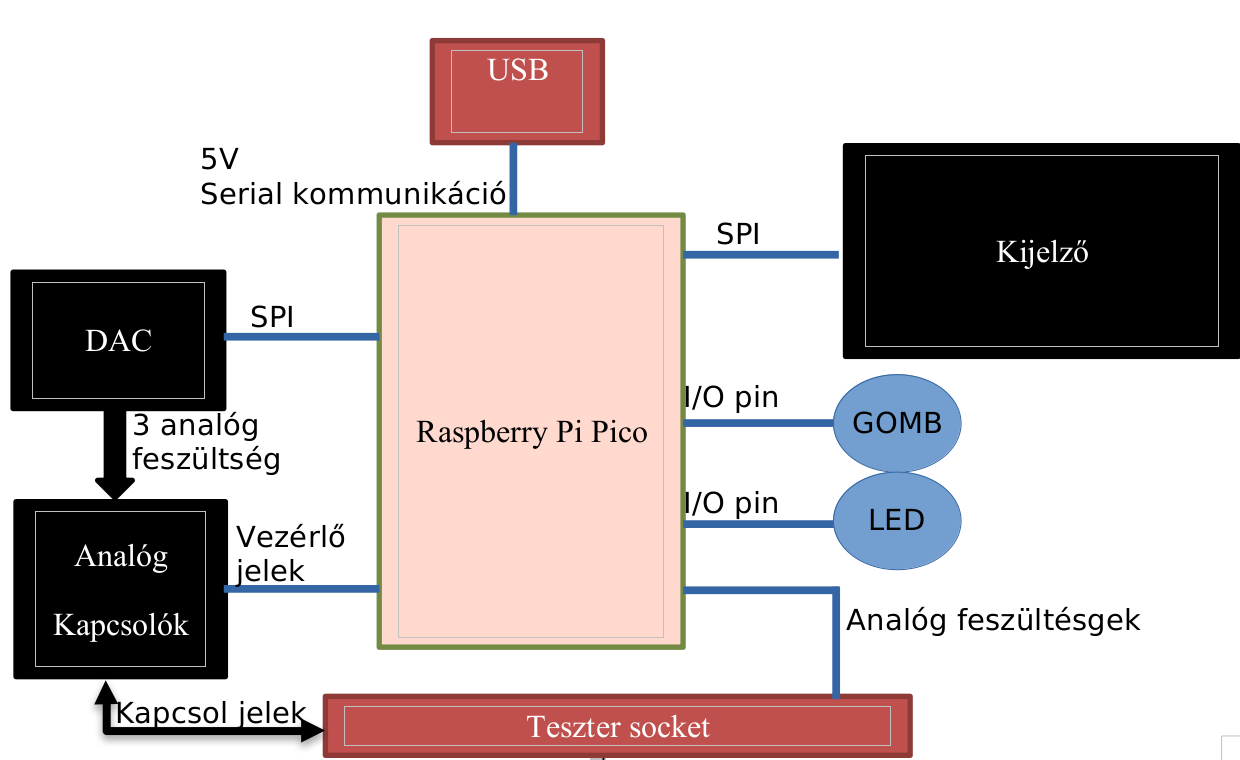
\includegraphics[scale=0.3]{images/literature/blockDiagramm.png}
    \caption{A rendszer blokk váza}
    \label{fig:blockDiagramm}
\end{figure}

\section{A rendszer osztály diagrammjai}

\subsection{Kijelző vezérlő}

Az alábbi ábrán[\ref{fig:displayClassDiagram}] a kijelző vezérlésért felelős osztályok láthatóak.
Ez a rendszer többi részétől elszigetelt rész, amely csupán 
megkapja az eredményeket a mérések után és megjeleníti azt.


\begin{figure}[H]
    \centering
    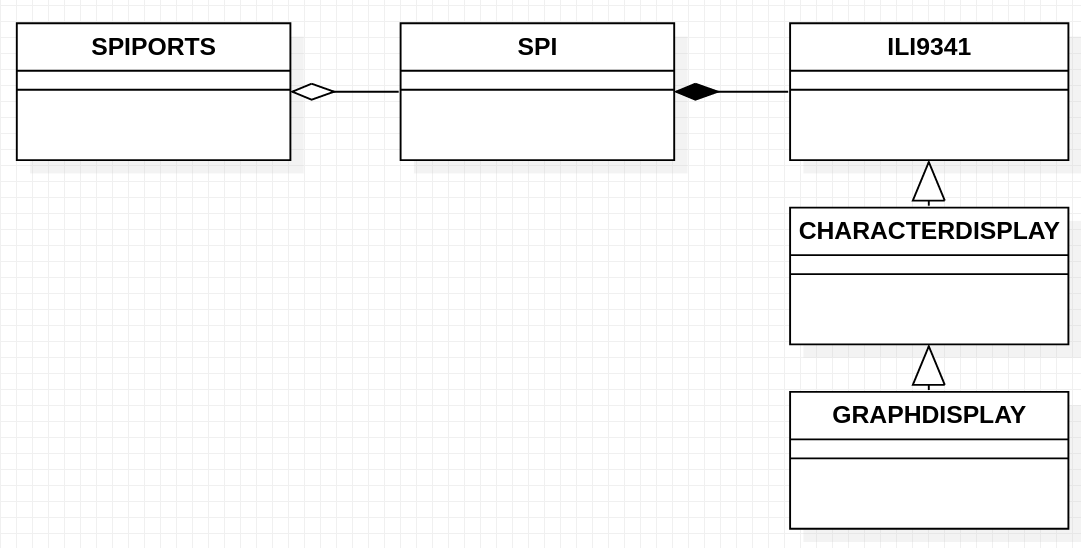
\includegraphics[scale=0.4]{images/diagrams/displayClassDiagram.png}
    \caption{A kijelző osztály diagramja}
    \label{fig:displayClassDiagram}
\end{figure}

Az ILI9341 osztály az alapszintű vezérlésért felelős, itt csak az 
adat küldési funkcionalitás és a képernyő inicializálása van
implementálva. A CHARACTERDISPLAY osztály kibővíti ezt és lehetővé
teszi egyszerű szöveg megjelenítését a kijelzőn.
A GRAPHDISPLAY kibővítve ezt képes megjeleníteni grafikont
a kijelzőre beépített skálázással, hogy lehetőleg az egész kijelzőt kihasználja.


\subsection{Mérő áramkör osztály diagrammja}

Alábbiakban [\ref{fig:ControlClassDiagram}] a rendszer az adatok méréséért felelős osztályai láthatóak,
ezek az osztályok alkotják a mérő eszközök vezérlését, mint a 
DAC és az analóg kapcsolók és az adatok mérését.
A rendszrben az ADC globális osztály és abból csak egy van.

\begin{figure}[H]
    \centering
    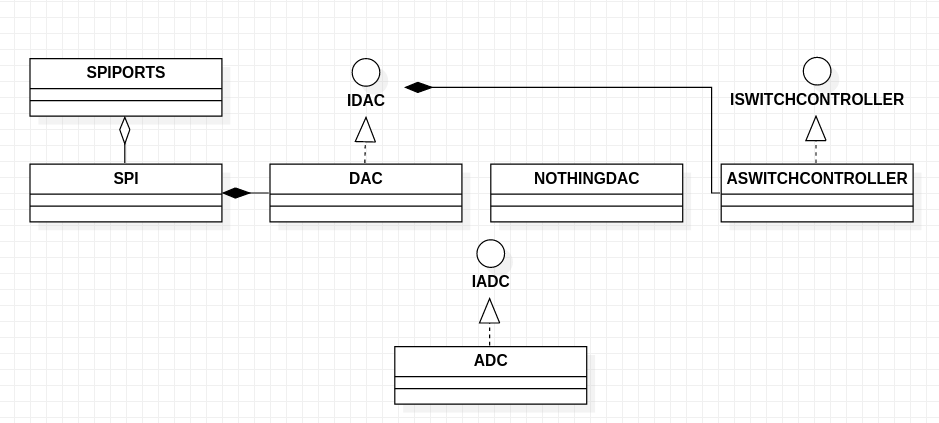
\includegraphics[scale=0.5]{images/diagrams/ControlClassDiagram.png}
    \caption{A vezérlő osztályok diagramja}
    \label{fig:ControlClassDiagram}
\end{figure}


\subsection{Számításokért felelő osztályok}

A következő osztályok[\ref{fig:CalculateClassDiagram}] felelnek a részeredmények kiszámításáért. A 
számításokat az ACALCULATE osztály végzi, az ADCCORRECTER osztály
feladata az ADC konstans hibájának a kiküszöbölésére. Az 
ISWITCHCONTROLLER az előző [\ref{fig:ControlClassDiagram}] ábrán látható
vezérlő rendszerrel van kapcsolatban. A BASEVALUES osztály a mérés során
történt ideiglenes adatok tárolására szolgál.


\begin{figure}[H]
    \centering
    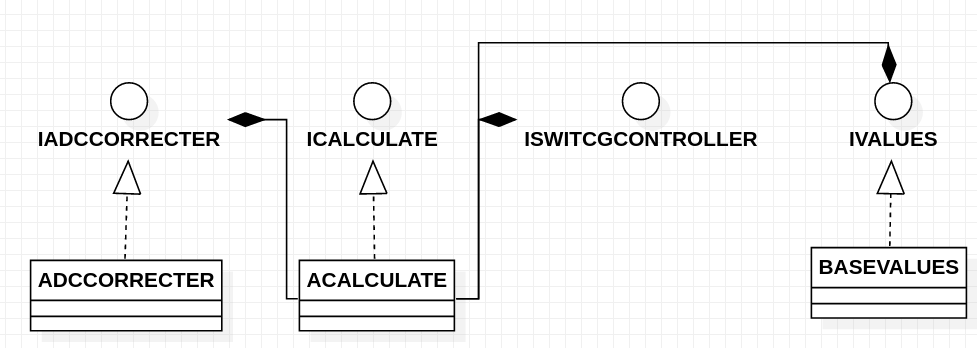
\includegraphics[scale=0.4]{images/diagrams/CalculateCalssDiagram.png}
    \caption{A számításokat elvégző osztályok diagramja}
    \label{fig:CalculateClassDiagram}
\end{figure}

\section{A mérés folyamat ábrája}

A mérés lépései a következőképpen történik[\ref{fig:CalculateStateDiagram}].
Első lépésben ellenállásra tesztel, ez ha nem talál semmit,
vagyis egyik teszter láb sincs csatlakoztatva, vagy nem reagál akkor 
a tesztelt komponens hibás, vagy nincs csatolva. Amennyiben valamilyen 
eszköz érzékelve van abban az esetben megpróbálja megmérni az ellenállás 
értékét, miközben figyelve arra, hogy ellenőrizzen lehetséges diódára is.
Ezt úgy oldja meg, hogy a dióda ellenállástól eltérően csak egy irányban vezet és
a feszültség esés konstans az áramerősségtől független.

Amennyiben dióda van detektálva abban az esetben a dióda útvonalon folyatódik a
tesztelés, különben megpróbálja megmérni az alkatrész kapacitását.

A dióda esetben ellenőrzi, hogy az alkatrész az 2 inverz dióda, és 
megméri a nyitó feszültségét. Amennyiben nem 2 inverz dióda, akkor abban az esetben
teszteli tranzisztorra is, ebben az lépésben képes az NPN és PNP tranzisztorokat
is detektálni és meghatározza a tranzisztor lábkiosztását.

\begin{figure}[H]
    \centering
    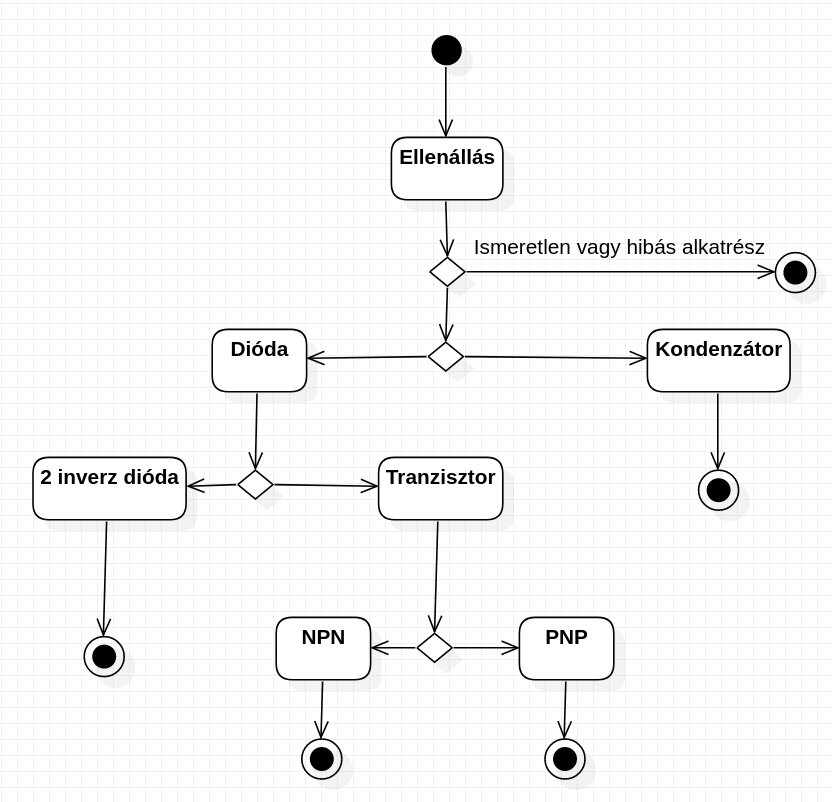
\includegraphics[scale=0.55]{images/diagrams/stateDiagram.png}
    \caption{A mérés fázisai}
    \label{fig:CalculateStateDiagram}
\end{figure}

%--------------------------------------------------------------------

\section{Mérő áramkör}

A rendszer hasonlóan épül fel, mint a példaként használt rendszer \cite{similarSystem}, viszont néhány módosítással.
Viszont az elméleti alapja hasonló. A komponens lábára egy ellenálláson keresztül feszültséget kapcsolva és a 
feszültség mérésével az ellenállás után meg lehet állapítani az áramerősséget és a feszültség esést a komponensen.
Ezekből az értékekből számítások segítségével ki lehet számolni, hogy mi az ismeretlen komponens (ennek a leírása
és lépései a későbbiekben lesznek részletezve) és értékét. A jelenlegi rendszer mérő áramkör része a következőkben
látható. [\ref{fig:ownTesterConnection}]

\begin{figure}[H]
    \centering
    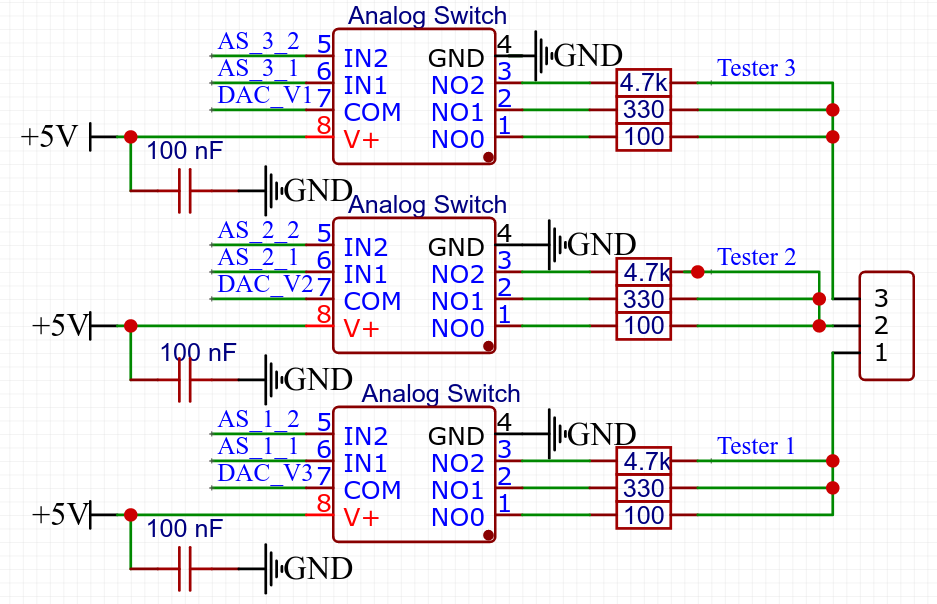
\includegraphics[scale=0.3]{figures/images/literature/TeszterConnections.png}
    \caption{Saját teszter bekötési rajza}
    \label{fig:ownTesterConnection}
\end{figure}

Ebben az esetben szükséges analóg kapcsolók használata, mivel az eredeti
teszter csak digitális jeleket használ amit direkt a GPIO-ról voltak kivezetve,
így az ellenállások közti váltásokért belsőleg a mikrovezérlő felel. Viszont ebben
az esetben a jelek analóg jelek amit egy külső DAC generál, így a mikrovezérlő nem
képes belsőleg kapcsolni ezeket ezért egy 3 kimenetes analóg kapcsoló van alkalmazva
erre a célra.

Mivel csak egy kapcsolón csak egy kimenet aktív egy időben, így az ellenállások után
a vezetékez összekapcsolhatóak, mivel azok nem fogják befolyásolni a rendszer működését,
erre a részre van kapcsolva az ADC egyik csatornája is, mivel itt a feszültség érték
azonos a komponens lábán található feszültséggel, így a komponenst nem kell módosítani,
hogy a feszültség látható legyen a lábán.

Az analóg jel 0V-3.3V közt lehetséges és a DAC maximálisan 50mA-t képes leadni, viszont
mivel a kondenzátorokat ki kell sütni csatlakoztatás előtt és külső tápfeszültség nem 
kapcsolható így a maximális áramerősség 33mA-nél nem lehet nagyobb semmilyen esetben.

A rendszer átlagolva nézi a feszültséget a komponens lábán, mellyel nagyobb pontosság
érhető el, mivel a zajok kevésbé befolyásolják a jelet. Viszont képes időben is mérni
a feszültséget, hogy hogyan változik a feszültség ahogy telik az idő. Az ADC mintavételezési sebessége 500ksps, 
viszont ez lelassítható egy belső késleltetővel. Ami segítségével
a lassan változó jelek is megfigyelhetőek, mint például egy nagy kondenzátor töltődése.

\section{A mérés menete a felhasználó által}

Az PCB-n található felhasználó által használható eszközök egy kapcsoló és a 
teszter socket ahová a komponenst kell helyezni. A kapcsoló egy kétállású
kapcsoló mely a mikrovezérlőt leállítja, vagy elindítja ami által a mérés
automatikusan elindul.

A rendszer tartalmaz 2 LED-et ami látható a következő fényképen is az
áramkörről is a kijelző jobb felső sarka fölött [\ref{fig:Aramkor}]. 
Amennyiben egyik LED sem világít, és a kijelző sem egy fehér hátteret
mutat abban az esetben a mikrovezérlő nem kap áramot, ilyenkor ellenőrizni
kell az USB kábelt.

Amennyiben a kijelző egy fehér képet mutat, viszont egyik LED sem világít akkor
a vezérlő reset állapotban van, ezt a vezérlő alatt levő kapcsoló ON 
pozícióba való állításával lehet orvosolni.

A mérés kezdetekor a piros LED felkapcsol, majd mérés befejeztekor a Zöld 
LED is felkapcsol, ebben az esetben a mérés sikeres volt és az eredmény meg 
kell jelenjen a kijelzőn és az USB-n keresztül elküldve a számítógéphez.

A teszter sockethez nem lehet tápforrást vagy elemet csatlakoztatni, ide tartoznak
a nagy méretű kondenzátorok is, a kis méretűeket képes kisütni, de ajánlott 
csatlakoztatás előtt kisütni ezeket is.

